%==============================================================================
%  Supplementary material — paper 1, the fire spread model
%  Target: International Journal of Wildland Fire (CSIRO Publishing)
%
%  IJWF wants supplementary items NUMBERED SEPARATELY from the main text and
%  SUBMITTED AS SEPARATE FILE(S) — hence a document of its own rather than an
%  appendix inside spread-paper.tex. Figures are S1..S5, equations S1..
%
%  Build with:  make supp     ->  build/supplementary.pdf
%
%  It shares references.bib and the patched ijwf.bst with the main paper, but
%  NOT the CSIRO class: that class is built for a full article (title block,
%  running heads, two columns, author statements) and none of it belongs here.
%
%  CROSS-REFERENCES INTO THE PAPER ARE HAND-MAINTAINED: the two documents share
%  no .aux, so "Eqn 5 of the main text" is a literal string, not a \ref. As of
%  2026-09-01 the paper's numbered equations are
%    1 flammability indices   2 the data model      3 the hierarchical mean
%    4 the parameter bounds   5 the covariance      6 the spatial overlap
%  and its figures are 1 study area, 2 spread curves, 3 parameters vs FWI,
%  4 vegetation effect, 5 burn probability, 6 DHARMa, 7 the regional validation.
%  Re-check these after any edit that adds or removes a numbered equation.
%
%  Contents follow the thesis's chapter 4 appendix (Barberá 2025), translated
%  and renotated to the manuscript's symbols: a_v/b_v/c_v for the flammability
%  coefficients (the thesis's alpha/beta/omega, which collided with the spread
%  coefficients), Phi for aspect, and VFI/TFI for IIV/IIT.
%==============================================================================

\documentclass[11pt,a4paper]{article}

% The figures come out of cairo_pdf as PDF 1.7; pdflatex defaults to 1.5 and
% warns on every inclusion. It includes them correctly either way.
\pdfminorversion=7

\usepackage[margin=2.5cm]{geometry}
\usepackage{graphicx}
\usepackage{amsmath}
\usepackage{booktabs}
\usepackage[round,authoryear]{natbib}
\bibpunct{(}{)}{;}{a}{}{;}
\usepackage[colorlinks=true,allcolors=blue]{hyperref}
\usepackage{caption}
\captionsetup{labelfont=bf,font=small}

\graphicspath{{figures/}{../figures/}}

% Supplementary numbering: Fig. S1, Eqn S1, Table S1.
\renewcommand{\thefigure}{S\arabic{figure}}
\renewcommand{\thetable}{S\arabic{table}}
\renewcommand{\theequation}{S\arabic{equation}}

\title{Supplementary material for\\
\textit{Fitting a hierarchical fire spread model with Approximate Bayesian
Computation}}
\author{Iv\'an Barber\'a}
\date{}

\begin{document}
\maketitle

\section{The flammability indices}
\label{sec:fi}

To parameterise the two flammability indices we modelled the probability that a
cell burned at least once over the period and study area of
\citet{barbera_patterns} (1999--2022, 24 fire seasons). The data were a random
sample of 9194 points taken in the burnable portion of the study area,
constrained to lie at least 800\,m apart. The model was

\begin{equation}
\label{eq:fimodel}
\begin{aligned}
    y_i &\sim \ \text{Bernoulli}(\theta_i) \\
    \text{logit}(\theta_i) &= a_{v[i]} + b_{v[i]} \, (\mathrm{NDVI}_i - c_{v[i]})
        + \delta_1 \, E_i + \delta_2 \, N_i + \delta_3 \, P_i \\[4pt]
    a_v &\sim \ \text{Normal}(\mu_a, \sigma_a) \\
    \log(-b_v) &\sim \ \text{Normal}(\mu_b, \sigma_b) \\
    \text{logit}(c_v) &\sim \ \text{Normal}(\mu_c, \sigma_c) \\[4pt]
    \mu_a &\sim \ \text{Normal}(0, 10), \qquad
    \sigma_a \sim \ \text{Normal}(0, 5)\text{T}[0, ] \\
    \mu_b &\sim \ \text{Normal}(\log(100), 2), \qquad
    \sigma_b \sim \ \text{Normal}(0, 2)\text{T}[0, ] \\
    \mu_c &\sim \ \text{Normal}(0, 5), \qquad
    \sigma_c \sim \ \text{Normal}(0, 3)\text{T}[0, ] \\[4pt]
    \delta_k &\sim \ \text{Normal}(0, 10), \qquad k \in \{1, 2, 3\},
\end{aligned}
\end{equation}

\noindent where $y_i \in \{0, 1\}$ indicates whether cell $i$ burned over the
study period, $\theta_i$ is its burn probability, $E$ is elevation, $N$ is
northness weighted by slope (Eqn~1 of the main text) and $P$ is slope. The three
topographic variables were standardized for fitting and their coefficients
transformed back to the original scale afterwards. The subscript $v[i]$ is the
vegetation type of cell $i$, numbered as in Table~1 of the main text. The
vegetation parameters $a$, $b$ and $c$ were given hierarchical priors so that
types with few data --- dry forest above all --- could be estimated; $b$ was
forced to be negative so that the effect of NDVI is unimodal, with $c_v$ the
NDVI at which burn probability peaks.

The slope coefficient $\delta_3$ is not part of the topographic flammability
index. It was included only to improve the estimation of the other parameters:
slope enters the spread model separately, and there it is \textit{directional},
since spread uphill and downhill differ. In Eqn~1 of the main text the two
indices are rescaled to mean 0 and standard deviation 1 over the dataset used
to fit this model. Fig.~\ref{fig:fi} shows the resulting indices as functions of
the variables that compose them.

\begin{figure}[htbp]
\centering
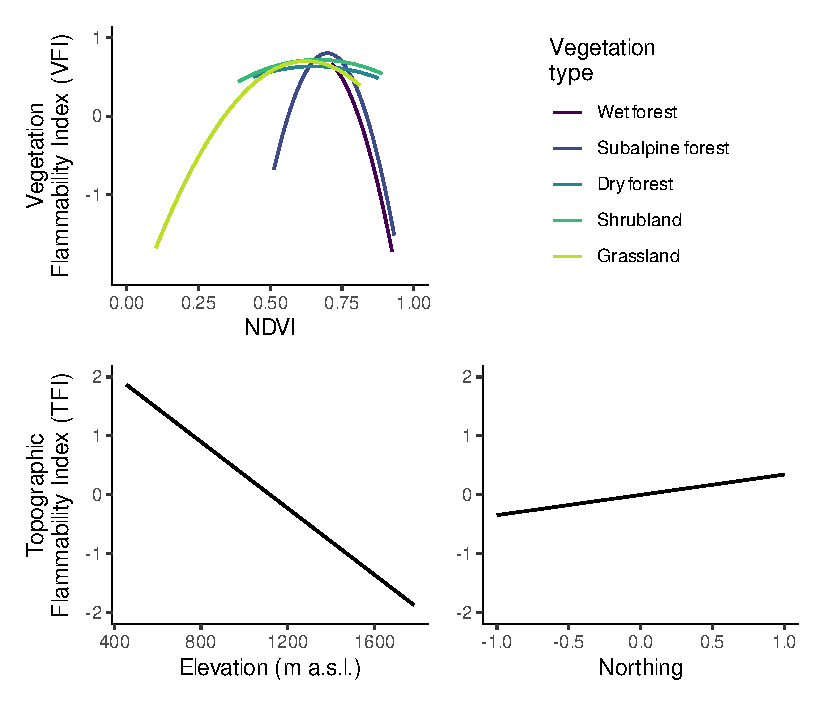
\includegraphics[width=0.85\textwidth]{figS1_flammability_indices}
\caption{The flammability indices as a function of the variables that compose
them, as defined in Eqn~1 of the main text. The vegetation flammability index
(VFI) is a unimodal function of NDVI whose position and curvature depend on
vegetation type; the topographic flammability index (TFI) decreases with
elevation and increases towards north-facing slopes. Each curve is drawn over
the range of the predictor observed for that vegetation type.}
\label{fig:fi}
\end{figure}

\section{The effect of vegetation type on spread probability as a function of
fire weather}
\label{sec:vegeffect}

One question the spread model is meant to answer is how the effect of
vegetation type on spread probability changes with fire weather. The
coefficient on VFI ($\beta_1$, Eqn~2 of the main text) did not vary with FWI
(Fig.~3 of the main text), but the nonlinearity of the logistic function means
that the effect of one variable on the probability depends on the values and
effects of the others, even with no interaction terms in the linear predictor.
This matters here because FWI does affect other coefficients, notably those
governing wind and slope. If a rising wind coefficient pushes spread
probability close to 1, the effect of vegetation should be attenuated, at least
for spread in the downwind direction. To evaluate this implicit interaction we
computed how the effect of vegetation type on spread probability changes with
FWI, propagating the effect of FWI on all six spread parameters.

To compare vegetation types we fixed elevation at 900\,m\,a.s.l.\ and aspect at
$90^\circ$ (northness $= 0$), which fixes TFI. To retain the directional effects
of slope and wind, and their joint variation over the landscape, we sampled 500
cells of the burnable area of Nahuel Huapi National Park, in the centre of the
study area, from the same raster used for simulation, which carries wind speed
and slope among other layers. To weigh uphill and downhill spread equally we
duplicated the set of cells and set slope to $0^\circ$ in the second half --- the
spread model assumes that downhill spread is like spread on flat ground
(Eqn~2 of the main text).

Comparing vegetation types also requires a VFI for each, and therefore an NDVI.
Because NDVI varies with topography, we predicted its expected value for the
topographic conditions analysed (the 500 sampled slopes, with elevation and
aspect fixed) with a generalized additive model with a Beta distribution for
NDVI rescaled to $[0, 1]$, fitted to the same dataset used for the flammability
indices (Section~\ref{sec:fi}) and with slope, elevation and aspect as
predictors. From this we obtained the expected NDVI at 900\,m\,a.s.l.\ on
east-facing slopes over all sampled slope values, and from it the VFI of each
vegetation type in every sampled cell.

With elevation and aspect fixed, and with the 500 sampled values of slope and
wind speed (plus the 500 with slope set to zero) and their VFI for each
vegetation type, we computed spread probability by vegetation type along a
sequence of FWI values, averaging the predictions over the sampled cells. The
predictions therefore condition on fixed values of elevation, aspect and
vegetation type and marginalize over the distribution of wind speed, slope and
NDVI in the landscape, always assuming that the wind blows in the direction of
spread. They also marginalize over the random effects, by simulation. The
effect of vegetation type (Fig.~4A of the main text) is the mean absolute
deviation across the five types, all weighted equally.

\section{Extended results}
\label{sec:extended}

\subsection{Spread probability against the raw predictors}

Fig.~2 of the main text shows spread probability as a function of the two
flammability indices. Fig.~\ref{fig:curvesraw} decomposes them into the
variables they are built from, so that the effect of NDVI within each
vegetation type, of elevation and of northness can be read directly.

\begin{figure}[htbp]
\centering
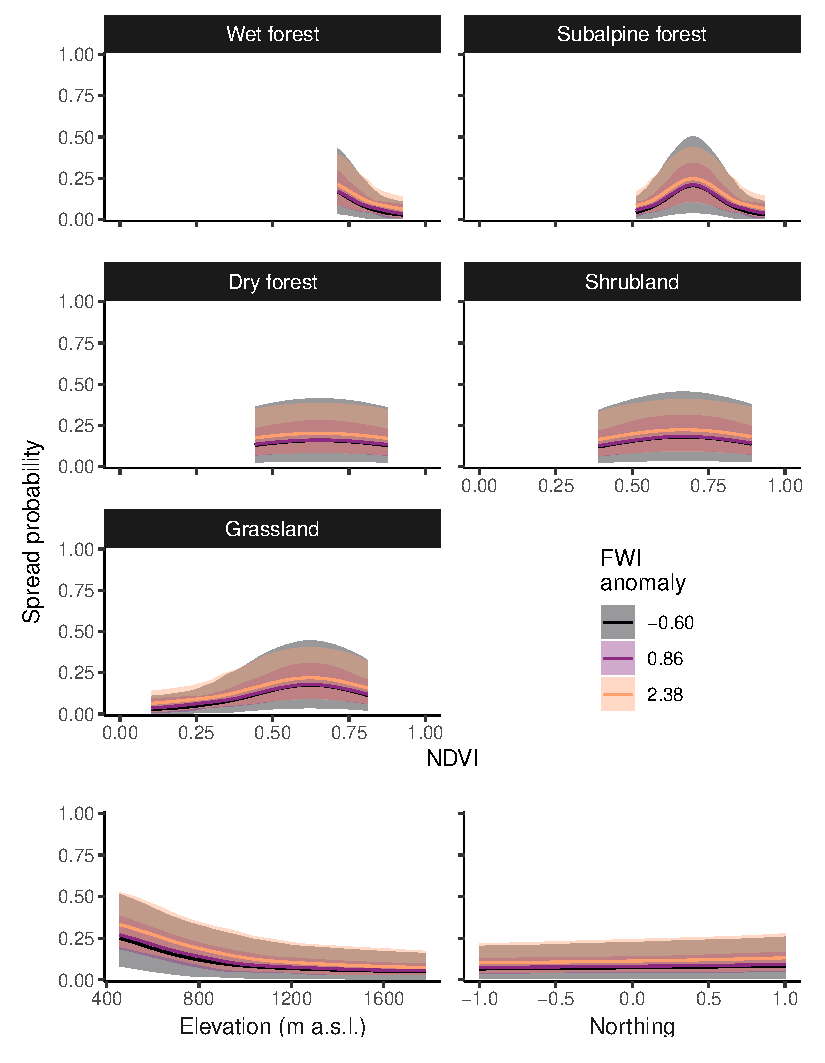
\includegraphics[width=0.8\textwidth]{figS2_spread_curves_raw}
\caption{Spread probability as a function of the predictors, decomposing the
vegetation and topographic flammability indices into the raw variables they are
built from, at the same three contrasting values of accumulated FWI used in
Fig.~2 of the main text (the mean and the 2.5th and 97.5th percentiles of the
mapped fires, on the original anomaly scale). Lines and bands are the mean and
the 95\,\% credible interval of the posterior. Each panel is drawn over the
range of the predictor observed for that vegetation type, which is why the NDVI
panels do not share an extent.}
\label{fig:curvesraw}
\end{figure}

\subsection{Correlation among the spread parameters}

Allowing the parameters to vary among fires also lets them covary.
Fig.~\ref{fig:corr} shows the posterior of the Pearson correlation between each
pair of parameters, computed on the scale the simulator uses rather than on the
unconstrained scale the multivariate normal is defined on, by simulating a full
set of fires from each posterior draw and back-transforming. Two distributions
are shown per pair. The one conditional on FWI fixes FWI at the mean of the
spread data and so represents the posterior of $\boldsymbol{\Omega}$ (Eqn~5 of
the main text); the marginal one lets each fire take its own FWI, and therefore
also carries any association induced by two parameters responding to fire
weather in the same, or in the opposite, direction. Where the two coincide, FWI
explains none of the association between that pair.

\begin{figure}[htbp]
\centering
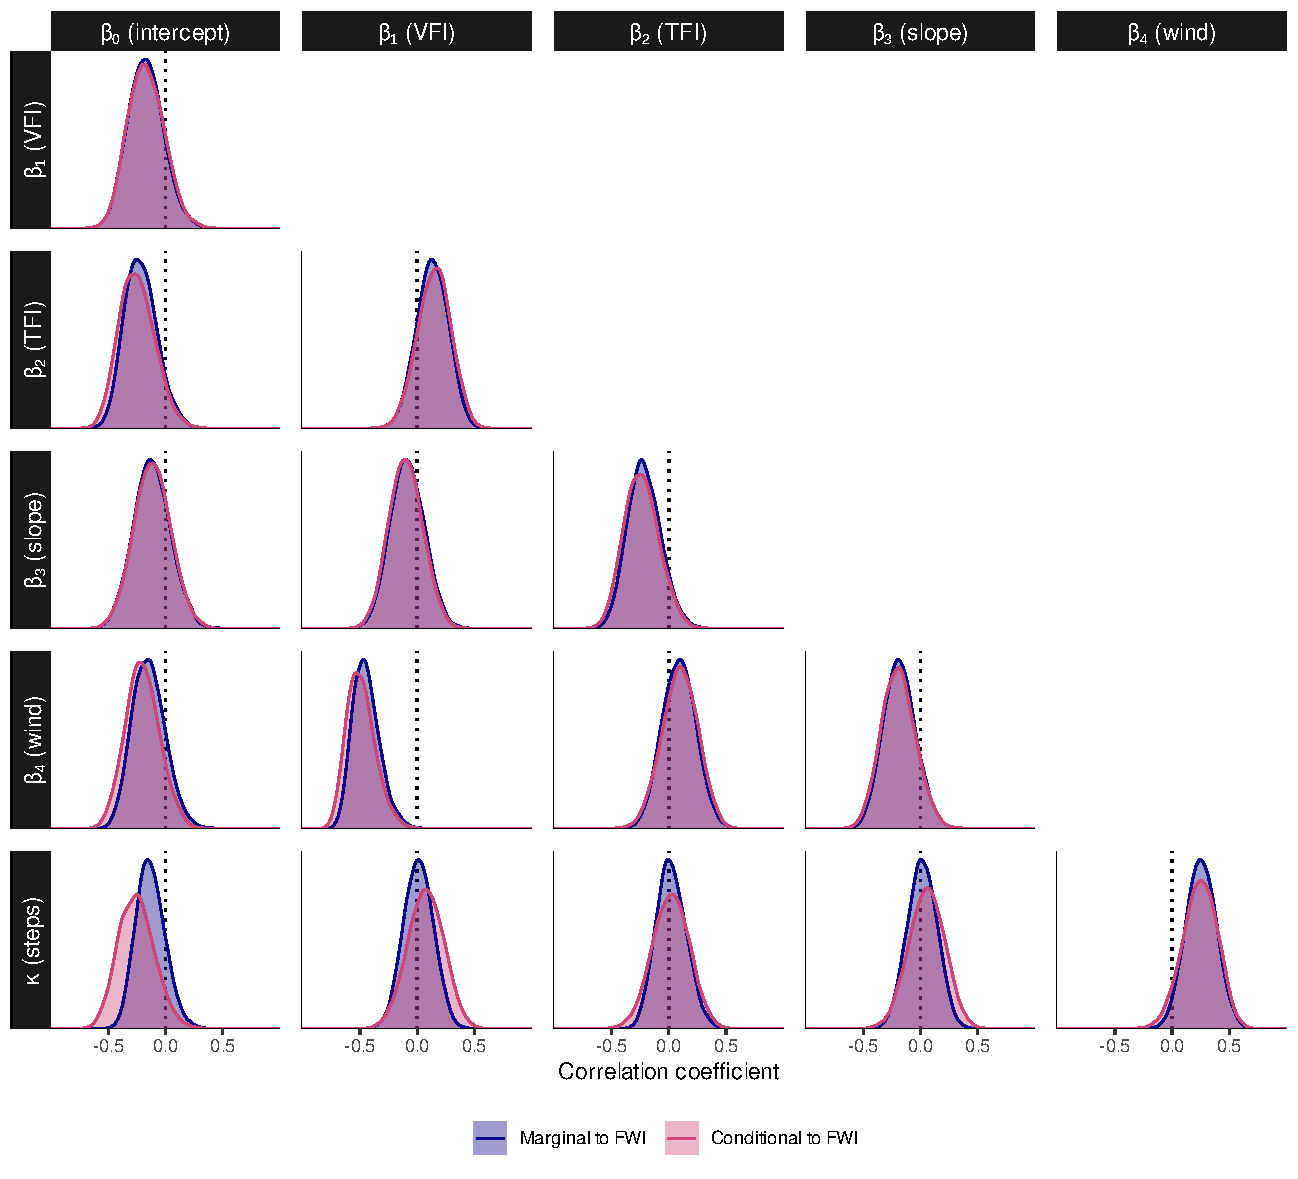
\includegraphics[width=\textwidth]{figS3_parameter_correlations}
\caption{Posterior distribution of the Pearson correlation coefficient between
each pair of spread parameters, marginal to or conditional on FWI. Coefficients
were computed by simulating parameter vectors from the fitted multivariate
distribution. The distributions conditional on FWI fix it at the mean of the
spread data and represent the posterior of $\boldsymbol{\Omega}$ (Eqn~5 of the
main text); the marginal ones include the effect of FWI, so that parameters
affected by it in a similar (or opposite) way show a marginal correlation of
larger (or smaller) magnitude than the conditional one.}
\label{fig:corr}
\end{figure}

\subsection{Fit to the mapped fires}

The two figures below describe the fit of the spread model to the 57 fires with
a known ignition point. As described in the main text, a parameter vector
$\boldsymbol{\beta}$ was estimated for each fire. Letting these parameters vary
among fires is how the model represents unobserved variables that matter for
fire: a fire put out quickly by crews or by rain may have a smaller number of
steps ($\kappa$) than average, and a fire that spread under a strong wind may
have a large wind coefficient ($\beta_4$). From the variation in
$\boldsymbol{\beta}$ among fires, and from how that variation relates to each
fire's FWI, we estimated a distribution of parameters (Eqn~3 of the main text),
which is what lets new $\boldsymbol{\beta}$ be simulated for hypothetical fires.

Model fit can therefore be assessed in two ways: with the parameters
\textit{fitted} to each fire, or with new parameters \textit{simulated} from the
estimated distribution. Simulated fires are expected to resemble the observed
ones more closely in the first case. In the second we are simulating fires that
differ from the observed ones precisely in the unobserved variables those
parameters absorb --- wind speed, suppression, rainfall and so on --- so the
comparison is not a test of the deterministic part of the model but a
measurement of how wide that distribution is. Each fire was simulated 2000 times
in each mode.

\begin{figure}[htbp]
\centering
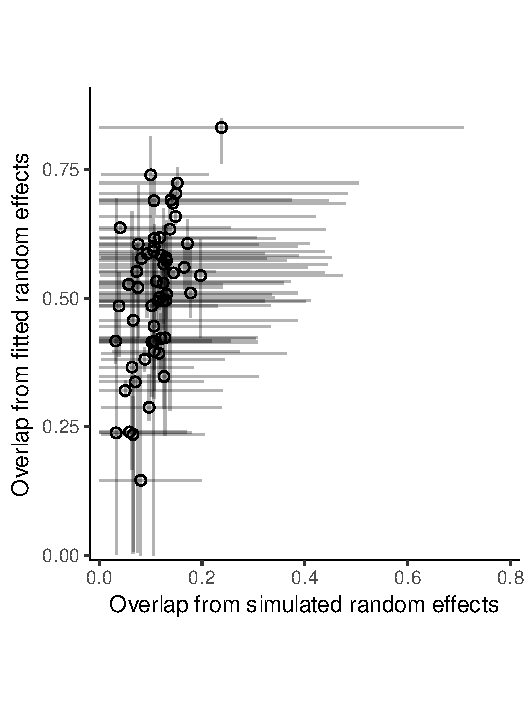
\includegraphics[width=0.5\textwidth]{figS4_overlap}
\caption{Spatial overlap (Eqn~6 of the main text) between simulated and observed
fires, using the parameters fitted to each fire or new parameters simulated from
the estimated distribution. Each point is one of the 57 fires with a known
ignition point; points and lines are the mean and the 95\,\% credible interval
of the posterior distribution of the overlap, approximated with 2000 simulations
per fire and per mode. Overlap under fitted parameters exceeds overlap under
simulated parameters for every one of the 57 fires.}
\label{fig:overlap}
\end{figure}

\begin{figure}[htbp]
\centering
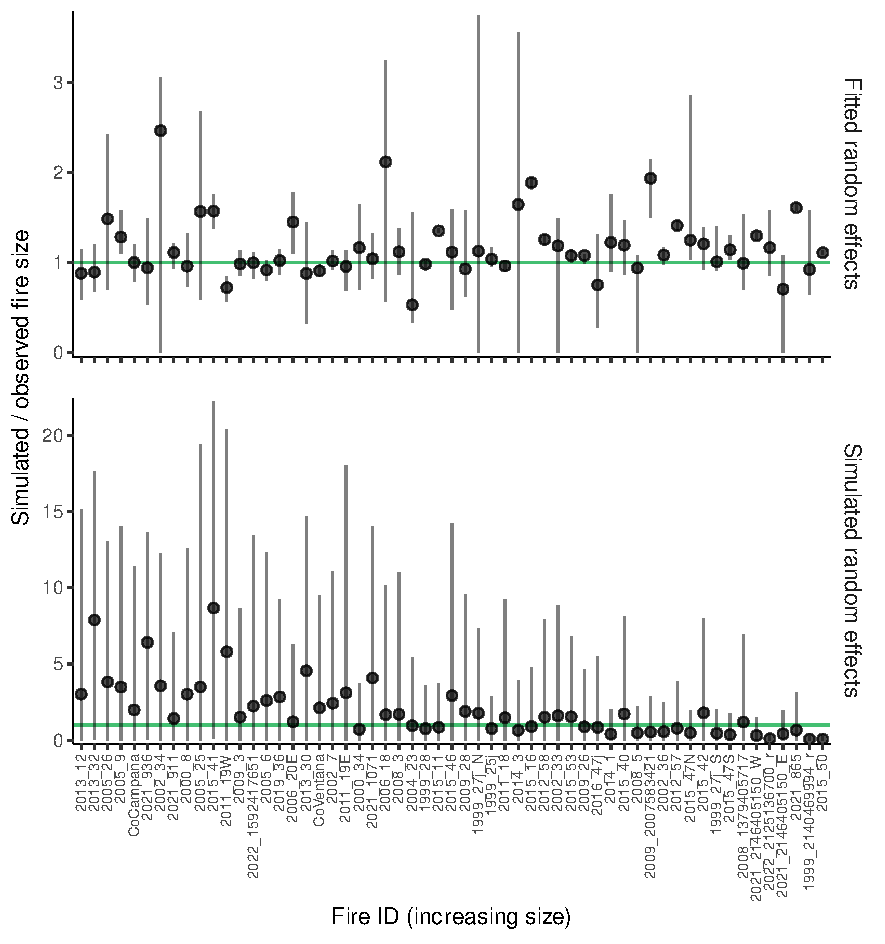
\includegraphics[width=0.9\textwidth]{figS5_size_quotient}
\caption{Ratio of simulated to observed fire size, using the parameters fitted
to each fire (top) or new parameters simulated from the estimated distribution
(bottom). Points and lines are the mean and the 95\,\% credible interval of the
posterior distribution of the ratio, approximated with 2000 simulations per
fire and per mode; the green line marks a ratio of 1. Fires are ordered by
observed size. Note the difference in the vertical scales.}
\label{fig:quotient}
\end{figure}

Although the model fits poorly when parameters are simulated, our aim was not a
simulator that predicts the advance of a particular fire, but one able to
generate fires similar to those that occur in the study area. The fit obtained
with simulated parameters is therefore not by itself a reason to reject the
model. Indeed, despite having been estimated with limited or no information on
atmospheric conditions and fire suppression, the model produces fires whose
sizes are of the same order as the observed ones (Fig.~\ref{fig:quotient}B).
Where it does fail --- fire shape --- the failure is structural, and is discussed
in the main text.

\bibliographystyle{ijwf}
\bibliography{references}

\end{document}
